\documentclass[12pt, oneside, a4paper]{article}
\usepackage[T1]{fontenc}
\usepackage[utf8]{inputenc}

%\usepackage[cp1251]{inputenc} % кодировка
\usepackage[english, russian]{babel} % Русские и английские переносы

\usepackage{cite}              % для корректного оформления литературы

\usepackage{graphicx}          % для включения графических изображений
\usepackage{enumitem}

\setlength{\emergencystretch}{3em}
\usepackage[hyphens]{url}
\usepackage[misc,geometry]{ifsym}

\usepackage[usenames]{xcolor}
\usepackage{soul}

\usepackage{amsmath}
\usepackage{amssymb}

\usepackage{algorithm}
\usepackage{algorithmic}

\usepackage{listings}

\usepackage{pavt-ru}
%\usepackage{pgfplots}
%\pgfplotsset{compat=1.9}
\usepackage{listings}


\lstset{
language=C,                 % выбор языка для подсветки (здесь это С)
basicstyle=\scriptsize\ttfamily, % размер и начертание шрифта для подсветки
numbers=left,               % где поставить нумерацию строк (слева\справа)
numberstyle=\tiny,           % размер шрифта для номеров строк
stepnumber=0,                   % размер шага между двумя номерами строк
numbersep=5pt,                % как далеко отстоят номера строк от подсвечиваемого кода
backgroundcolor=\color{white}, % цвет фона подсветки - используем \usepackage{color}
showspaces=false,            % показывать или нет пробелы специальными отступами
showstringspaces=false,      % показывать или нет пробелы в строках
showtabs=false,             % показывать или нет табуляцию в строках
frame=single,              % рисовать рамку вокруг кода
tabsize=2,                 % размер табуляции по умолчанию равен 2 пробелам
captionpos=t,              % позиция заголовка вверху [t] или внизу [b] 
breaklines=true,           % автоматически переносить строки (да\нет)
breakatwhitespace=false, % переносить строки только если есть пробел
escapeinside={\%*}{*)}   % если нужно добавить комментарии в коде
}

%Содержимое документа
\begin{document}

\title{Отчет о выполнении 3 задания практикума кафедры СКИ}
\authors{Р.М.~Куприй, 323 группа}
\organizations{Факультет ВМК МГУ имени М.В.~Ломоносова}

\section{Задание}

По заданию написана программа для решения системы линейных уравнений $Ax = b$, с разреженной матрицей $A$ и плотными векторами $x$, $b$. Система решается итерационным методом сопряженных градиентов (Conjugate Gradient Method) без предобуславливателя.

Итерационный метод решения заключается в последовательном уменьшении невязки и вычислении поправок к выбранному начальному приблежению решения. Алгоритм останавливается по достижению заданного максимального числа итераций либо при достижении невязки меньшей либо равной $10^{-12}$.

В программе реализована параллельная версия алгоритма с использованием технологий OpenMP.

\section{Методика тестирования}

В программе замеряется время разложения матрицы и время решение системы обратным ходом Гаусса, общее время есть сумма этих двух составляющих. Для верификации результатов вычисляется невязка решения: $||Ax - b||$, а также при известном решении системы -- невязка ошибки: $||x - solution||$. Примером известного решения может быть единичный вектор $x$, который возникает тогда, когда вектор $b$ составлен из сумм строк матрицы $A$.

Для тестирования производительности использовалась параллельная вычислительная система Polus, с 3 вычислительными узлами, в каждом из которых 2 10~ядерных процессора IBM POWER8. Для компиляции использовался компилятор \texttt{xlc++} с флагом опимизации -O5. Запуски проводились с равномерным выделением ядер для программы и их закреплением с помощью команды \texttt{\#BSUB -R affinity(core=x)} и специального предоставленного скрипта для запуска.

Для исключения выбросов и получения равномерной оценки по запускам, программа запускалась 6 раз для каждого замера. В каждом запуске проводилось от 3 до 10 разогревочных решений системы уравнений и от 5 до 50 отслеживаемых решений. По прогонам внутри каждого запуска выбиралось среднее время работы алгоритма, а среди всех запусков выбиралось минимальное. Получены резльтаты для разреженных матриц разного размера, при использовании 1, 2, 4, 8, 32, 64 нитей соотвественно.

\section{Оценки эффективности OpenMP программы}

При измерениях использовались расчетные сетки по кубикам со стороной 25, 50, 100 и 250. Соответственно, размер матрицы это третья степень размера стороны куба. Для каждого набора входных данных приведены графики общего времени решения системы, ускорения и эффективности.

Для маленькой сетки, на кубике со стороной 25, максимальное ускорение достигается на 8 и 16 нитях, при этом эффективность ускорения резко падает с ростом числа нитей~(Графики~\ref{fig:m25}). Алгоритм сходится за 58 итераций, достигается точность $10^{-13}$.

\begin{figure}[h!]
\center{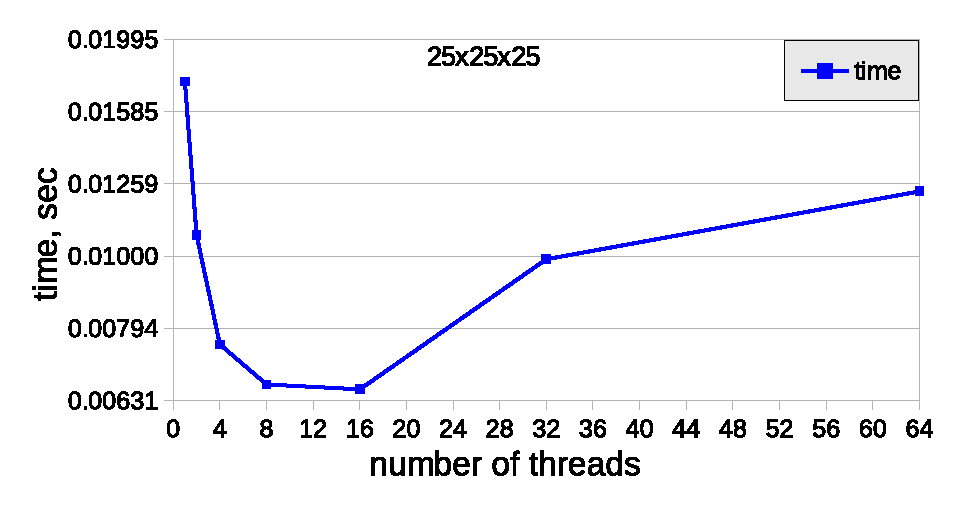
\includegraphics[width=12cm]{./pics/time25.eps}}
\center{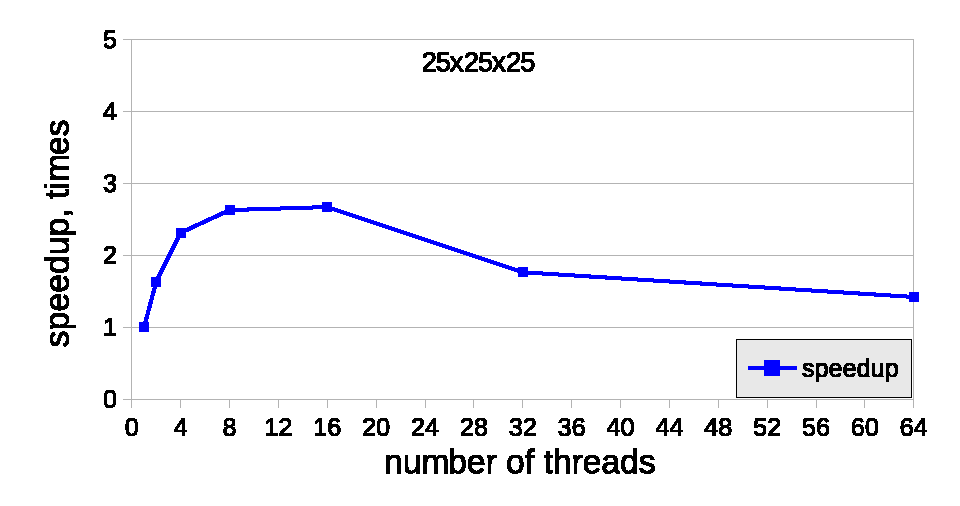
\includegraphics[width=12cm]{./pics/speedup25.eps}}
\center{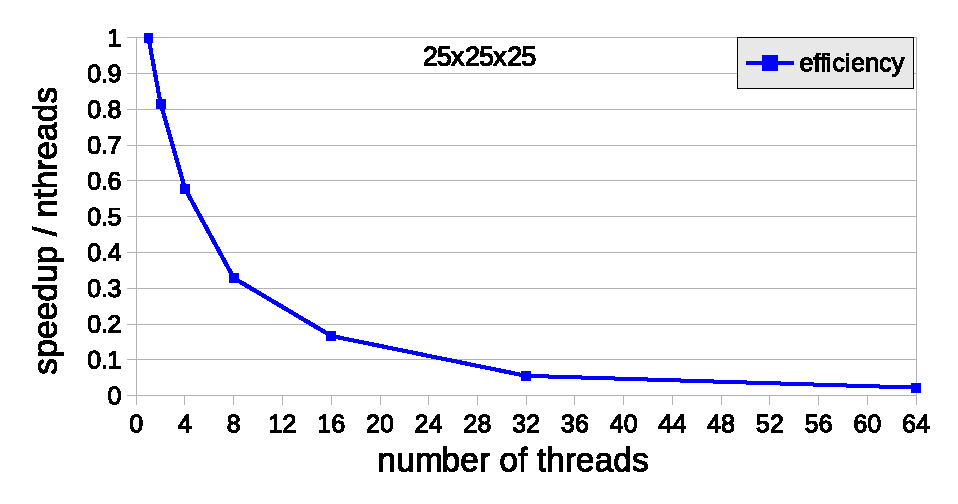
\includegraphics[width=12cm]{./pics/efficiency25.eps}}
\caption{Результаты распараллеливания программы для матрицы размером $25^3$; верхний график -- времена исполнения, срений -- достигаемое ускорение, нижний -- эффективность ускорения работы программы.}
\label{fig:m25}
\end{figure}

В следующем наборе измерений использовалась сетка кубика со стороной 50. C ростом объема данных растёт ресурс параллелизма, который можно использовать. Это повышает эффективность распараллеливания для заданного числа нитей. Максимальное ускорение также достигается на 16 нитях~(Графики~\ref{fig:m50}). Алгоритм сходится за 70 итераций, достигается заданная точность.

\begin{figure}[h!]
\center{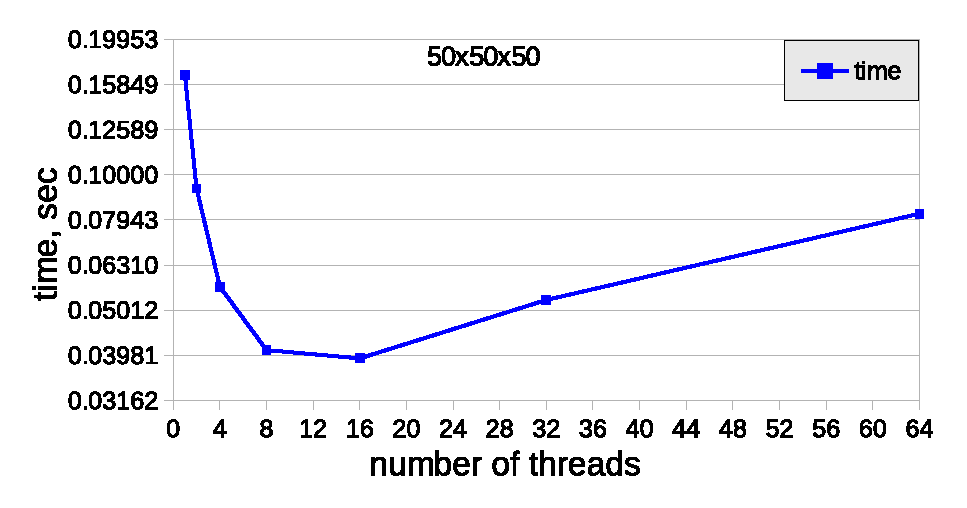
\includegraphics[width=12cm]{./pics/time50.eps}}
\center{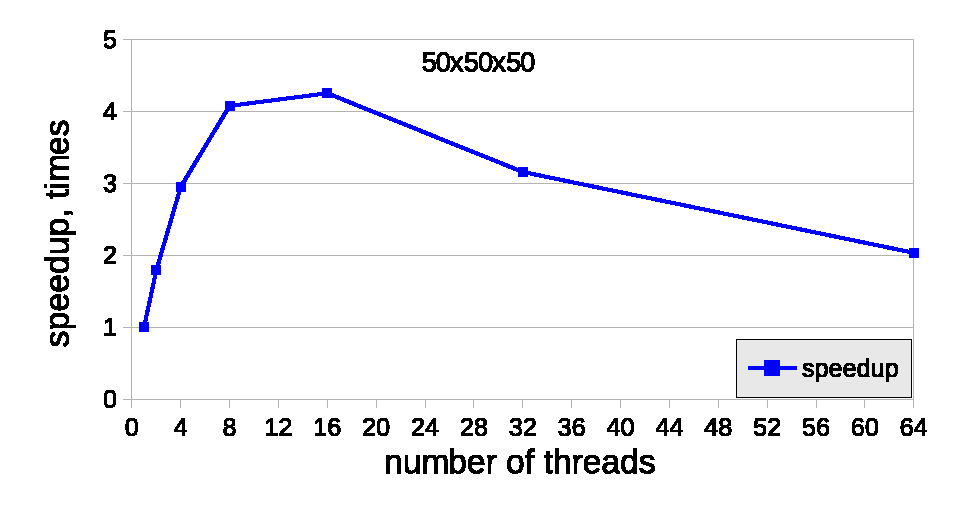
\includegraphics[width=12cm]{./pics/speedup50.eps}}
\center{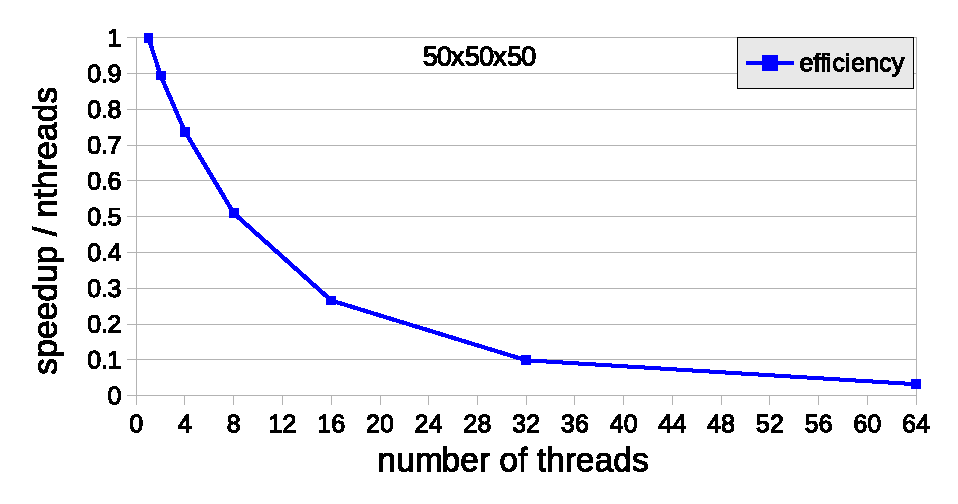
\includegraphics[width=12cm]{./pics/efficiency50.eps}}
\caption{Результаты распараллеливания программы для матрицы размером $50^3$; верхний график -- времена исполнения, срений -- достигаемое ускорение, нижний -- эффективность ускорения работы программы.}
\label{fig:m50}
\end{figure}

Набор данных входных данных среднего размера использует для построения системы сетку кубика со стороной 100. На этом датасете достигается максимальное ускорение на 16 нитях~(Графики~\ref{fig:m100}). Алгоритм сходится за 92 итерации.

\begin{figure}[h!]
\center{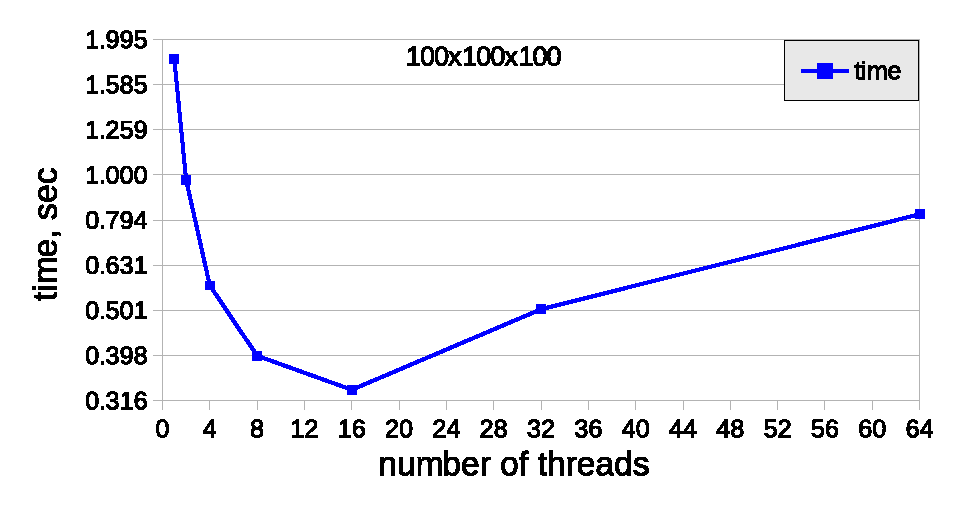
\includegraphics[width=12cm]{./pics/time100.eps}}
\center{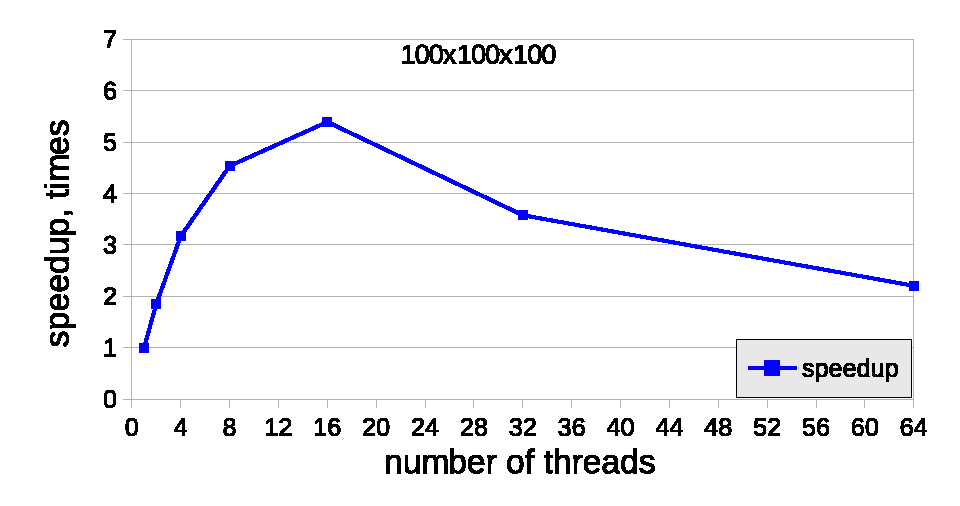
\includegraphics[width=12cm]{./pics/speedup100.eps}}
\center{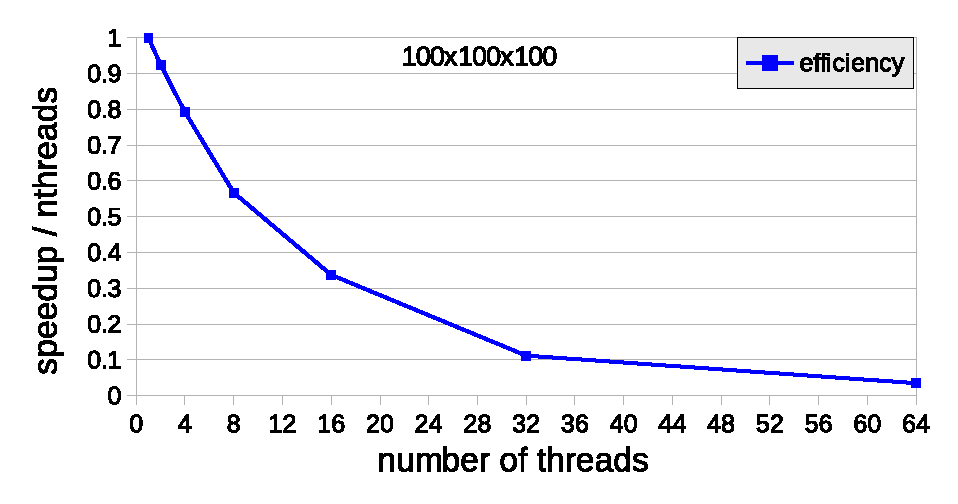
\includegraphics[width=12cm]{./pics/efficiency100.eps}}
\caption{Результаты распараллеливания программы для матрицы размером $100^3$; верхний график -- времена исполнения, срений -- достигаемое ускорение, нижний -- эффективность ускорения работы программы.}
\label{fig:m100}
\end{figure}

Для крупного набора входных данных используется кубик со стороной 250. На этом датасете максимальное ускорение достигается на 16 процессах~(Графики~\ref{fig:m250}).
Алгоритм сходится за 110 итераций.

\begin{figure}[h!]
\center{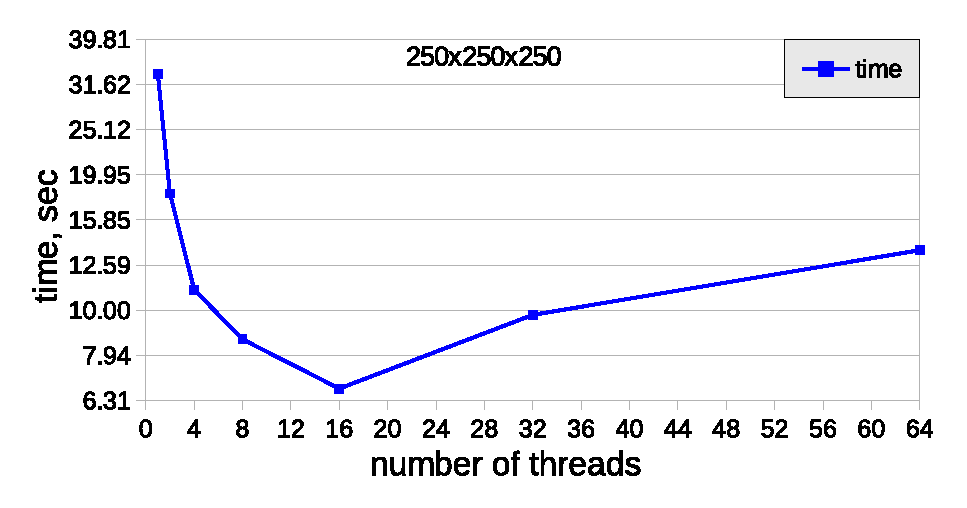
\includegraphics[width=12cm]{./pics/time250.eps}}
\center{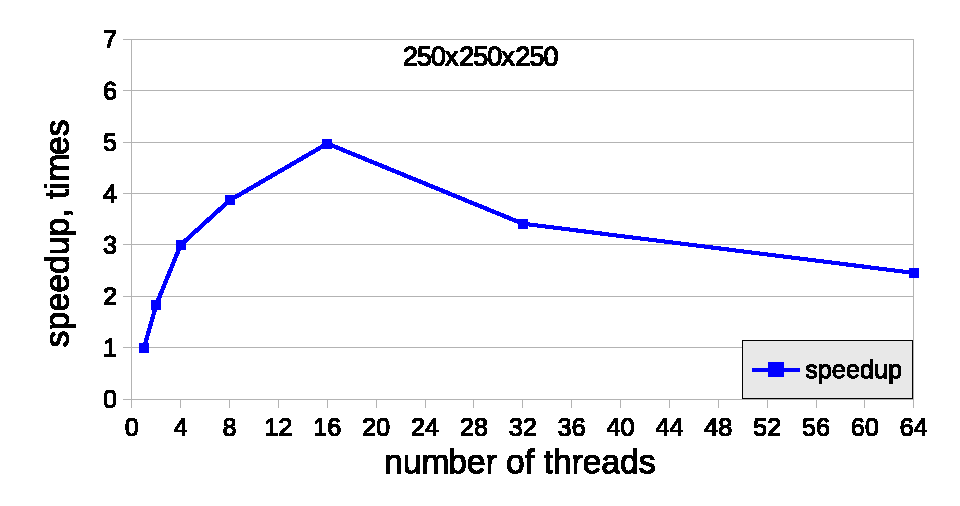
\includegraphics[width=12cm]{./pics/speedup250.eps}}
\center{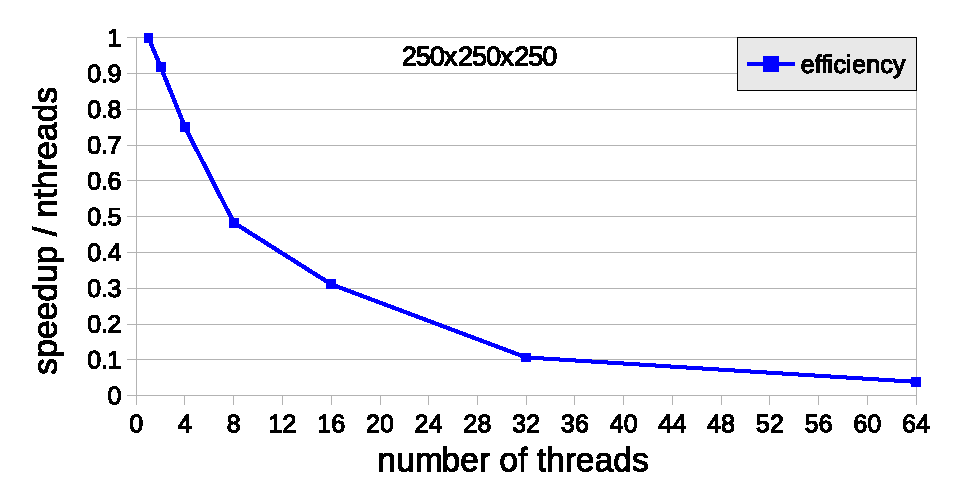
\includegraphics[width=12cm]{./pics/efficiency250.eps}}
\caption{Результаты распараллеливания программы для матрицы размером $250^3$; верхний график -- времена исполнения, срений -- достигаемое ускорение, нижний -- эффективность ускорения работы программы.}
\label{fig:m250}
\end{figure}

%Для очень крупного набора входных данных используется кубик со стороной 500. Максимальное ускорение достигается на 16 и 32 нитях~(Графики~\ref{fig:m500}). Ускорение немного ниже, чем на крупном датасете.

%\begin{figure}[h!]
%\center{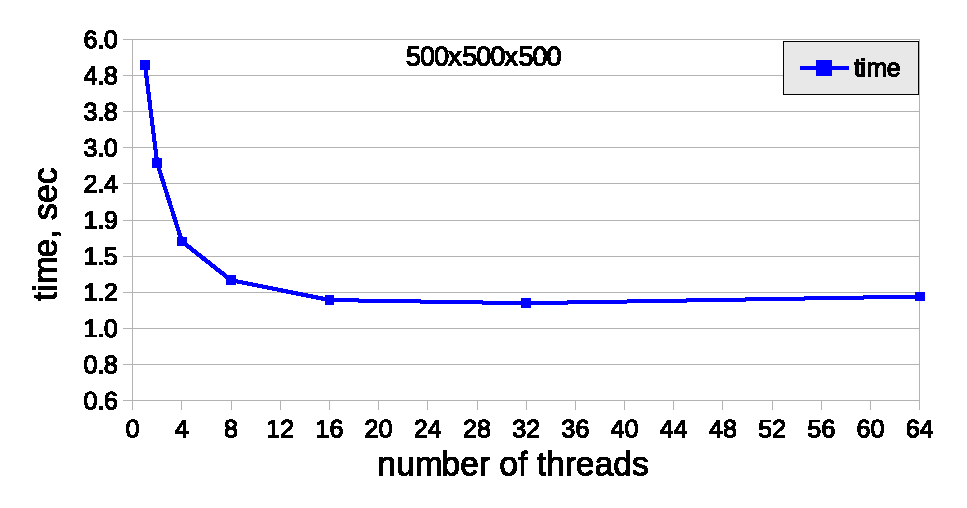
\includegraphics[width=12cm]{./pics/time500.eps}}
%\center{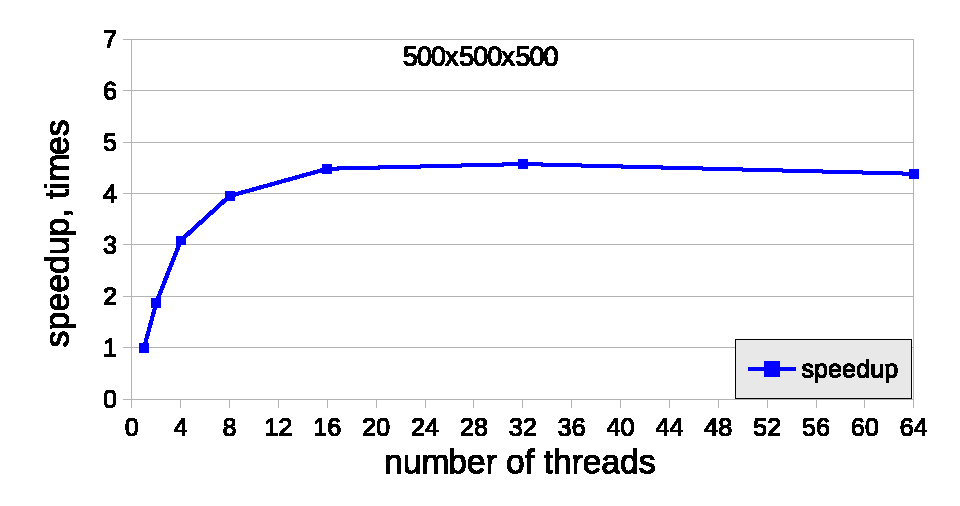
\includegraphics[width=12cm]{./pics/speedup500.eps}}
%\center{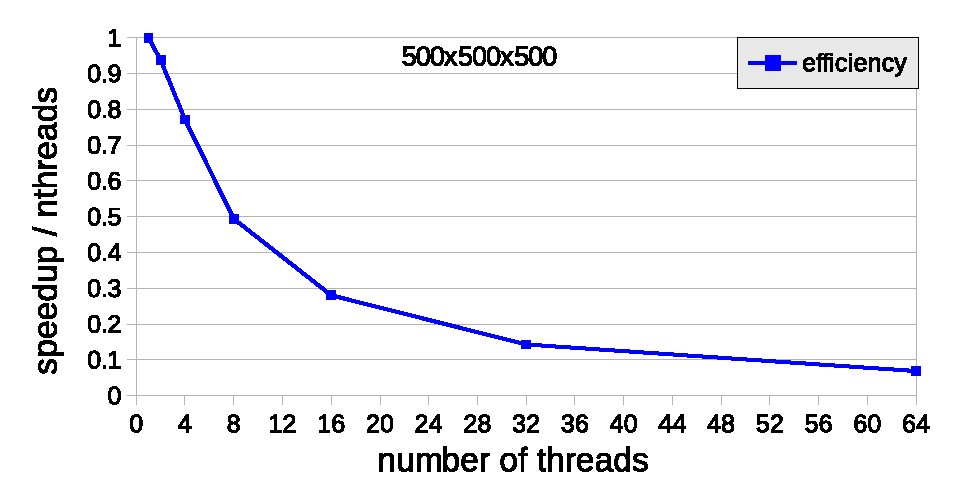
\includegraphics[width=12cm]{./pics/efficiency500.eps}}
%\caption{Результаты распараллеливания программы для матрицы размером $500^3$; верхний график -- времена исполнения, срений -- достигаемое ускорение, нижний -- эффективность ускорения работы программы.}
%\label{fig:m500}
%\end{figure}

\section{Анализ полученных результатов}

В результате всех измерений наблюдаются одинаковое поведение ускорения и эффективности. Эффективность резко падает с ростом числа нитей. Однако, для крупных размеров входных данных эффективность снижается плавнее.

Максимальное ускорение достигается на 8 или 16 нитях, при дальнешем росте числа нитей, ускорение резко падает.

Для верификации результатов также вычислялись невязки ошибки и решения, которые составляли порядок $10^{-11} - 10^{-13}$.

\subsection{Оценка производительности базовых операций}

Проведены дополнительные тесты для оценки производительности базовых операций \texttt{dot}, \texttt{axpby}, \texttt{SpMV}. Во всех вычислениях использовался тип \texttt{double} для хранения переменных в памяти. Вычисления проводились на кластере с пиковой производительностью $55.84\ TFlops$, с пропускной способностью шины памяти в узле $20\ GB/s$.

Производительность операции \texttt{dot} составляет $1.74\ GFlops$, или $0.006\%$ от пиковой производительности. Для этой операции, на каждом шаге внутреннего цикла есть 1 операция сложения и умножения и 2 операции чтения из памяти. Если считать прибавление результата умножения к переменной накопителю за операцию с регистровой памятью и не учитывать её, то вычислительная интенсивность операции \texttt{dot} равна $0.125$. Соответствующее значение TBP составляет $2.5\ GFlops$.

Производительность операции \texttt{axpby} достигает $2.77\ GFlops$. У этой операции во внутреннем цикле есть 2 операции умножения и 1 операция сложения на 2 или 3 операции чтения/записиси даннных в память. Таким образом вычислительная интенсивность этой операции составляет $0.1875$, а TBP равна $3.75\ GFlops$.

Операция SpMV показывает производительность в $3.3\ GFlops$. На каждой итерации у этой операции есть 1 сложение и умножение для операций с элементами массивов и по 2 операции сложения и умножения с индексами циклов. Также есть 4 операции чтения/записи в память. Если допустить, что индексы циклов хранятся в регистровой памяти, то вычислительная интенсивность приблизительно равна $0.2$, а TBP равна $4\ GFlops$.

Эти оценки позволяют оценить порядок эффективности выполнения операций на рассматриваемой системе.

\end{document}